\section{Giới thiệu}

\subsection{Bối cảnh}

Cơ chế attention là thành phần cốt lõi của Transformer. Trong mỗi lớp attention, điểm số giữa các vị trí được chuẩn hoá theo hàng bằng hàm softmax trước khi nhân với giá trị. Với độ dài chuỗi $L$, mỗi hàng cần $L$ phép tính $e^{x}$, $L-1$ phép cộng và một phép chia, và điều này lặp lại theo số hàng và số đầu attention. Khi mô hình được lượng tử hoá sang INT8, phần tính softmax trở thành điểm nghẽn nếu vẫn dùng số thực dấu phẩy động.

\subsection{Mục tiêu}

Đề tài xây dựng một bộ tăng tốc softmax theo hàng, trong đó toàn bộ phép tính dùng số nguyên, nhận đầu vào INT8 có dấu và trả về đầu ra UINT8 với scale $1/256$. Bộ tăng tốc được hiện thực dưới dạng IP Avalon-MM slave trên kit DE10-Standard (Cyclone V 5CSXFC6D6F31C6), dùng Quartus Prime Lite 18.1.

Các mục tiêu cụ thể:
\begin{itemize}
  \item Số học bit-exact so với một golden model viết bằng Python.
  \item Tần số hoạt động từ 100 MHz trở lên sau Fitter.
  \item Tổng số ALUT và DSP vượt 1000 theo yêu cầu môn học.
  \item Chạy được trên board qua JTAG và System Console, không cần Linux.
\end{itemize}

\subsection{Phạm vi}

Báo cáo tập trung vào thiết kế lõi \texttt{smx\_core}, gồm thanh ghi điều khiển, bộ đệm X/Y, bộ điều khiển và datapath. Wrapper Avalon, hệ thống Platform Designer và script demo do nhóm hiện thực đảm nhiệm; báo cáo mô tả các phần này ở mức giao diện và cấu trúc hệ thống (Chương 4). Phần kiểm thử lõi do nhóm kiểm thử thực hiện qua cổng \texttt{acc\_*}; kế hoạch và kết quả được trình bày ở Chương 6. Hình \ref{fig:smx-system} cho thấy vị trí của lõi trong hệ thống demo và ranh giới giữa các phần việc.

\begin{figure}[htbp]
  \centering
  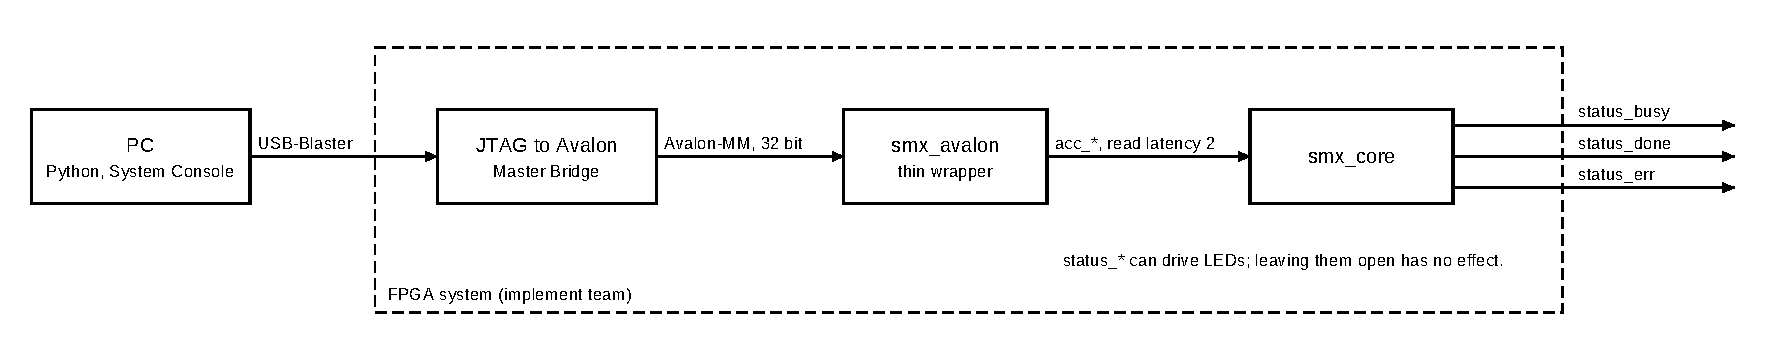
\includegraphics[width=\textwidth]{smx_system.pdf}
  \caption{Ranh giới hệ thống: PC, cầu JTAG to Avalon Master, lớp bao \texttt{smx\_avalon} và lõi \texttt{smx\_core}. Phần trong khung nét đứt nằm trên FPGA.}
  \label{fig:smx-system}
\end{figure}

Đề tài không bao gồm phép nhân ma trận, convolution, LayerNorm, GELU và masking. Hàm sigmoid và GELU chỉ được xem là mở rộng tuỳ chọn sau khi lõi hoàn thành.

\subsection{Đóng góp}

Các đóng góp chính của đề tài gồm:
\begin{enumerate}
  \item Thuật toán softmax thuần số nguyên, không dùng hàm log trong datapath, nhờ đưa hệ số $\log_2 e$ vào $K$ do phần mềm tính sẵn.
  \item Kết hợp IntMax với chuẩn hoá trực tuyến để chỉ cần hai lượt quét và hiệu chỉnh tổng bằng phép dịch.
  \item Tính lại $E$ ở lượt thứ hai từ bộ đệm đầu vào, thay vì lưu kết quả trung gian.
  \item Golden model bit-exact và đặc tả giao diện, làm cơ sở để các nhóm khác tích hợp và kiểm thử.
  \item Lõi RTL đã kiểm thử bit-exact với golden model và đạt mục tiêu tần số, tài nguyên sau Fitter.
\end{enumerate}

\subsection{Tóm tắt kết quả}

Bảng \ref{tab:summary} tóm tắt các kết quả chính của đề tài ở cấu hình mặc định; chi tiết và điều kiện đo nằm ở các chương được dẫn trong bảng.

\begin{table}[htbp]
\centering
\small
\begin{tabular}{lll}
\toprule
Hạng mục & Kết quả & Chương \\
\midrule
Cấu hình mặc định & $P = 8$ lane, $N_{\text{SEG}} = 8$, $L_{\max} = 512$, $R_{\max} = 16$ & 3, 4 \\
Sai số so với softmax float64 & khoảng 0,002, bằng nửa LSB của đầu ra & 3 \\
Tài nguyên sau Fitter & 1\,681 ALUT, 24 DSP, 21 khối M10K & 7 \\
Tần số tối đa & 122 đến 134 MHz qua ba seed & 7 \\
Độ trễ một hàng, $L = 512$ & 182 chu kỳ & 6, 7 \\
Kiểm thử lõi & 7 testcase, 458\,837 phép so, khớp bit-exact & 6 \\
Chạy trên board & [Chưa đo] & 7 \\
\bottomrule
\end{tabular}
\caption{Tóm tắt kết quả chính ở cấu hình mặc định.}
\label{tab:summary}
\end{table}

\subsection{Cấu trúc báo cáo}

Chương 2 khảo sát các hướng softmax phần cứng hiện có. Chương 3 đặc tả thuật toán và số học. Chương 4 mô tả kiến trúc hệ thống và giao diện. Chương 5 trình bày thiết kế từng khối. Chương 6 trình bày kế hoạch và kết quả kiểm thử. Chương 7 trình bày kết quả tổng hợp và đánh giá. Chương 8 kết luận và nêu hướng phát triển.
